\section{Événements utilisés}\label{chapter-ML-section-evt_gen}
%Utiliser les mêmes données simulées que dans les analyses de physique afin d'entraîner les modèles introduirait un biais.
L'objectif est de reconstruire la masse des particules se désintégrant en paire de leptons~\tau.
Il s'agit donc d'une tâche de régression.
Dans l'optique d'une utilisation dans les analyses telles que celle présentée dans le chapitre~\refChHTT,
il a été choisi d'utiliser des événements
$\higgsML\to\tau\tau$
où \higgsML\ est le boson de Higgs du modèle standard \higgs\ dont la masse est modifiée,
à l'instar de ce qu'ont fait \citeauthor{BARTSCHI201929}~\cite{BARTSCHI201929}.
La cible du modèle est donc la masse $m_{\higgsML}$.
\subsection{Génération avec \FASTSIM}\label{chapter-ML-section-evt_gen-FASTSIM}
Nous avons généré nos propres données simulées~\cite{fastsim_ece}
afin d'obtenir
une distribution continue des valeurs de $m_{\higgsML}$
et suffisamment d'événements pour chaque point de masse.
Dans le contexte de la collaboration CMS, nous avons utilisé \FASTSIM~\cite{FastSim_2011,FastSim_2014,FastSim_2017_1,FastSim_2017_2}.
Cet outil permet de procéder à l'ensemble de la simulation des événements introduite chapitre~\refChLHCCMS,
de la génération du processus physique à la reconstruction des objets physiques par le détecteur.
\par
Les données simulées correspondent à des collisions de protons
avec une énergie dans le centre de masse de \SI{13}{\TeV}.
Les processus physiques sont générés par
\PYTHIA~8~\cite{pythia8.2}
avec les réglages CUEP8M1~\cite{tunes_2016,tunes_2019}.
La production du boson \higgsML\ se fait par fusion de gluons,
il s'agit du mode de production dominant dans le cas du boson de Higgs du modèle standard \higgs.
De plus, le rapport de branchement $\BR(\higgsML\to\tau\tau)$ est fixé à 1,
\ie\ que \higgsML\ se désintègre forcément en paires de leptons~\tau.
Tous les événements obtenus sont donc bien du type $\higgsML\to\tau\tau$.
\par
La masse de \higgsML\ varie de \num{50} à \SI{800}{\GeV} par pas de \SI{1}{\GeV}.
Il est important d'utiliser l'intervalle le plus étendu possible, il correspond à la gamme utile des modèles obtenus.
L'effet de l'étendue de cet intervalle est discuté dans la section~\ref{chapter-ML-section-discussion}.
\par
Il n'est pas possible, par la méthode que nous utilisons, de générer des événements avec $m_{\higgsML}\gtrsim\SI{1}{\TeV}$.
Cela est dû à la largeur $\Gamma_{\higgs}$ de \higgs, représentée figure~\ref{fig-_Higgs_xsec_book_3-SM_Width} en fonction de $m_{\higgs}$.
\begin{figure}[b]
\centering

\subcaptionbox{Largeur du boson de Higgs du modèle standard~\cite{Higgs_xsec_book_3}.\label{fig-_Higgs_xsec_book_3-SM_Width}}[.45\textwidth]
{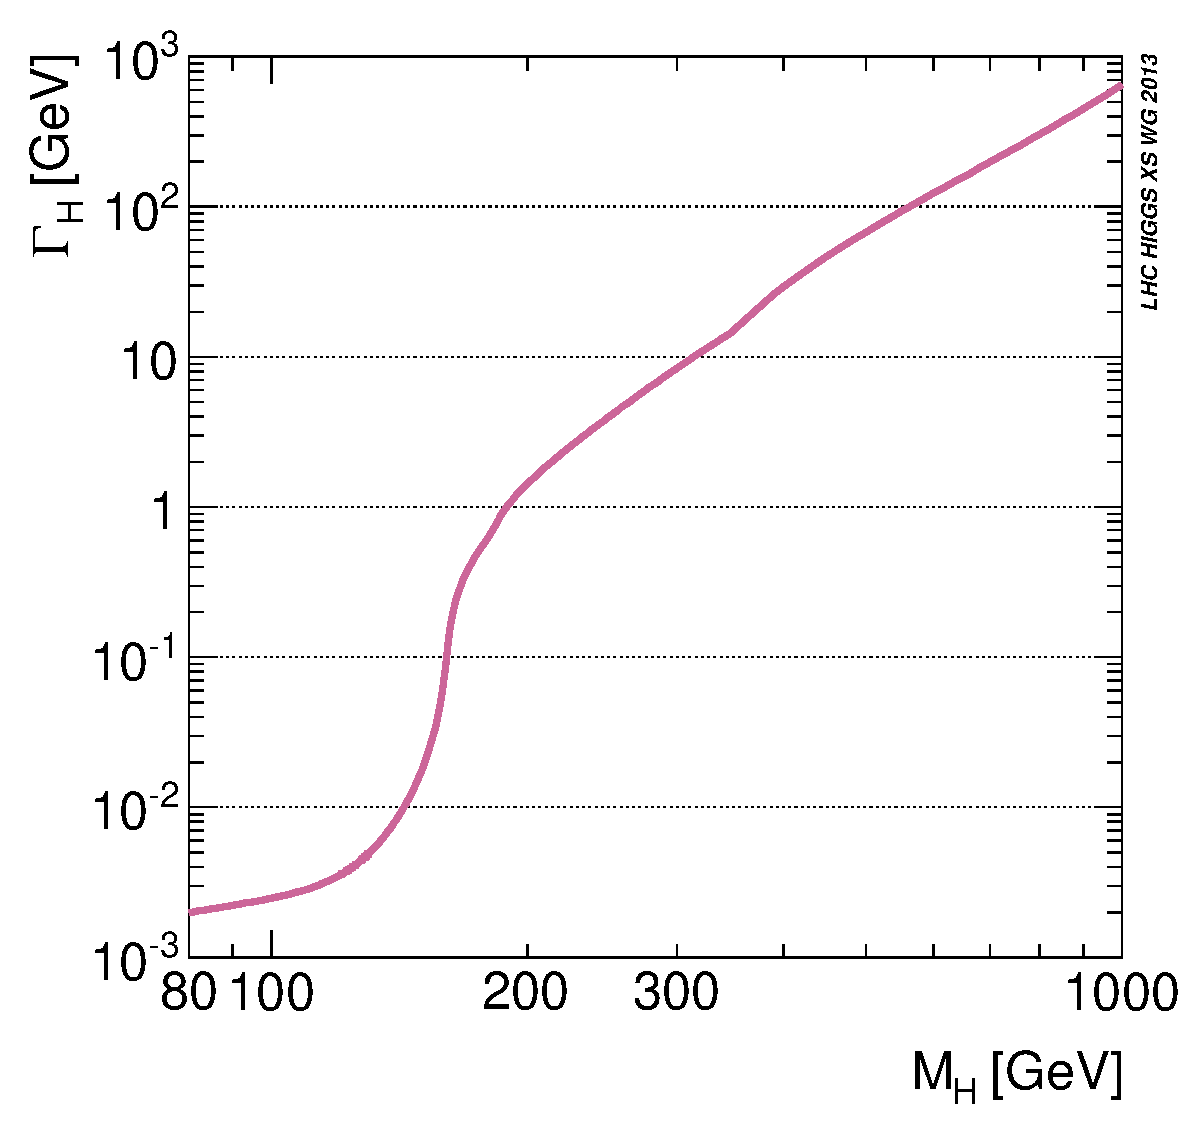
\includegraphics[width=.45\textwidth]{\PhDthesisdir/plots_and_images/from_Higgs_xsec_book_3/SM_Width.pdf}}
\hfill
\subcaptionbox{Efficacité de sélection des événements pour $m_{\higgsML}\in\llbracket \num{50} , \num{800} \rrbracket \usp \SI{}{\GeV}$ dans les différents canaux et pour tous les canaux.\label{fig-analysis_cuts_efficiency}}[.45\textwidth]
{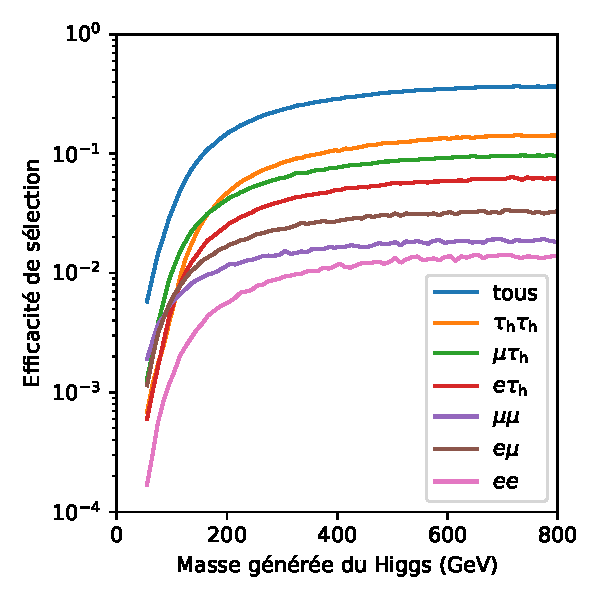
\includegraphics[width=.45\textwidth]{\PhDthesisdir/plots_and_images/my_plots/ML/from_ML_plots/FastSim_NanoAOD_to_NN/ALL_PU2017/plots_Htt_merged_NanoAODSIM_ALL_PU2017-DeepTau_1000/analysis_cuts_efficiency.pdf}}

\caption{Origine des limites haute (gauche) et basse (droite) de l'intervalle de masse utilisé.}
\end{figure}
La largeur d'une particule est liée à sa durée de vie $\tau$ selon
\begin{equation}
\Gamma = \frac{\hbar}{\tau}
\mend
\end{equation}
Ainsi, plus une particule se désintègre rapidement, plus sa largeur est importante.
Le principe de Heisenberg mène alors à une incertitude sur la masse, due à la durée de vie $\tau$, égale à $\Gamma$.
Or, vers \SI{1}{\TeV}, $\Gamma_{\higgsML}\simeq m_{\higgsML}$.
C'est pourquoi la génération de tels événements est compromise avec \higgsML\ défini comme \higgs\ avec une masse modifiée.
Nous générons donc uniquement des événements en-deçà de \SI{800}{\GeV}.
\par
%Bien qu'il soit possible pour une particule de se désintégrer en deux~\tau\ dès que sa masse est plus élevée que $2\,m_{\tau} = \SI{3.5}{\GeV}$,
La sélection des événements est présentée dans la section~\ref{chapter-ML-section-evt_gen-selection}.
Son efficacité est représentée sur la figure~\ref{fig-analysis_cuts_efficiency}.
Plus de \SI{99}{\%} des événements sont rejetés lorsque $m_{\higgsML} < \SI{50}{\GeV}$.
Nous ne considérerons donc pas de masse plus basse.
\par
S'il est possible d'appliquer des poids aux événements afin d'équilibrer l'entraînement sur l'ensemble des valeurs de la cible,
plus d'événements sont générés à basse masse afin d'obtenir des topologies d'événements variées malgré la faible efficacité de sélection.
Ainsi, la quantité d'événements générés pour chaque valeur de $m_{\higgsML}$ est de:
\begin{itemize}
\item \num{60000} pour $ \SI{50}{\GeV} \leq m_{\higgsML} < \SI{300}{\GeV} $;
\item \num{20000} pour $ \SI{300}{\GeV} \leq m_{\higgsML} < \SI{500}{\GeV} $;
\item \num{10000} pour $ \SI{500}{\GeV} \leq m_{\higgsML} \leq \SI{800}{\GeV}$.
\end{itemize}
\par
L'empilement est modélisé par superposition du signal $\higgsML\to\tau\tau$ à des événements dits de \og biais minimum \fg~\cite{pythia8.2}.
Il s'agit d'événements pouvant contenir des interactions dures, mais n'activant pas de \HLTpath.
La quantité d'empilement ajoutée à l'événement $\higgsML\to\tau\tau$ suit le profil d'empilement de l'année 2017.
Les conditions des collisions simulées sont ainsi identiques à celles de l'année 2017 au LHC.
\subsection{Sélection des événements}\label{chapter-ML-section-evt_gen-selection}
\subsubsection{Jets}
À l'instar de l'analyse présentée au chapitre~\refChHTT,
les jets sont
soumis à la procédure de CHS~\cite{CMS-PAS-JME-14-001} décrite dans le chapitre~\refChJERC\
et
reconstruits par l'algorithme anti-\kT~\cite{Cacciari_antikT} avec un paramètre $R=\num{0.4}$.
Ces jets doivent également passer les critères d'identification présentés dans le chapitre~\refChLHCCMS.
L'identification des jets issus de quarks~\quarkb\ (\quarkb-\emph{tagging}) est réalisée par l'algorithme \DeepCSV~\cite{Sirunyan_heavy_flavor_jets_2018,DeepJet}.
Les jets tels que $\pT > \SI{20}{\GeV}$ et $\abs{\eta}<\num{2.5}$ sont considérés comme issus d'un \quarkb\ si leur score est supérieur à \num{0.3033}.
Les jets non identifiés comme issus d'un \quarkb\ ne sont retenus que si $\pT > \SI{30}{\GeV}$ et $\abs{\eta}<\num{4.7}$.
\subsubsection{Canaux \tauh\tauh, \mu\tauh, \ele\tauh\ et \ele\mu}
Dans le cas des canaux
\tauh\tauh, \mu\tauh, \ele\tauh\ et \ele\mu,
la sélection des événements se fait comme exposé dans le chapitre~\refChHTT\ pour l'année 2017.
Afin d'obtenir un modèle dont les prédictions auront non seulement un sens dans les régions de contrôle et de détermination, les coupures sur
\begin{itemize}
\item $\mT^{(\mu)}$ dans le canal \mu\tauh;
\item $\mT^{(\ele)}$ dans le canal \ele\tauh;
\item $\Dzeta$ dans le canal \ele\mu
\end{itemize}
ne sont pas appliquées.
La construction du dilepton est inchangée.
La correspondance des objets du dilepton avec ceux ayant activé le \HLTpath\ n'est pas vérifiée.
%\par
%En plus des canaux listés ci-dessus, nous avons également sélectionné des événements des canaux \mu\mu\ et \ele\ele,
%selon les procédures présentées ci-après.
\renewcommand{\IfMoreOnePair}{Si plus d'une paire possible existe dans l'événement, une seule est retenue selon la logique exposée dans le chapitre~\refChHTT.}
\subsubsection{Canal \mu\mu}
\paragraph{Sélection des muons}
\AllSatisfyingFollowing{muon}{$L_1$ ou $L_2$}:
\begin{itemize}
    \item $\pT^{\mu} > \SI{10}{\GeV}$;
    \item $\abs{\eta^{\mu}} < 2.4$;
    \item \Leptondzdxy;
    \item \RelIsoBelow{\mu}{0.15};
    \item passer le \MediumMuonID.
\end{itemize}
\paragraph{Sélection du dilepton}
\AtLeastOneOSPair{\mu\mu}
\DeltaRPair{0.3}
\IfMoreOnePair
\paragraph{Vétos de leptons supplémentaires}
\LeptonVetoes
\begin{itemize}
    \item \LeptonVetoesExtraMuonMuMu;
    \item \LeptonVetoesExtraEle, l'électron devant \PassConversionVeto\ et \LessTwoMissingHitsVertex.
\end{itemize}
\subsubsection{Canal \ele\ele}
\paragraph{Sélection des électrons}
\AllSatisfyingFollowing{électron}{$L_1$ ou $L_2$}:
\begin{itemize}
    \item $\pT^{\ele} > \SI{20}{\GeV}$;
    \item $\abs{\eta^{\ele}} < 2.4$;
    \item \Leptondzdxy;
    \item \RelIsoBelow{\ele}{0.1};
    \item passer le \NinetyNineEleMVA.
\end{itemize}
\paragraph{Sélection du dilepton}
\AtLeastOneOSPair{\ele\ele}
\DeltaRPair{0.5}
\IfMoreOnePair
\paragraph{Vétos de leptons supplémentaires}
\LeptonVetoes
\begin{itemize}
    \item \LeptonVetoesExtraMuon;
    \item \LeptonVetoesExtraEleEleEle, l'électron devant \PassConversionVeto\ et \LessTwoMissingHitsVertex.
\end{itemize}
\subsection{Événements obtenus et pondération}
Plus de 22 millions d'événements ont été générés.
Environ 3 millions sont sélectionnés selon les critères présentés précédemment.
La distribution de $m_{\higgsML}$ dans ces événements sélectionnés est représentée sur la figure~\ref{subfig-distribution-inclusive-Higgs_mass_gen-raw-all_events}.
Quelques événements présentent des valeurs de $m_{\higgsML}$ au-delà de \SI{800}{\GeV}, cet effet est dû à la largeur de cette particule,
représentée sur la figure~\ref{fig-_Higgs_xsec_book_3-SM_Width} en fonction de sa masse.
\begin{figure}[h]
\centering

\subcaptionbox{Distribution brute sur tous les événements.\label{subfig-distribution-inclusive-Higgs_mass_gen-raw-all_events}}[0.45\textwidth]
{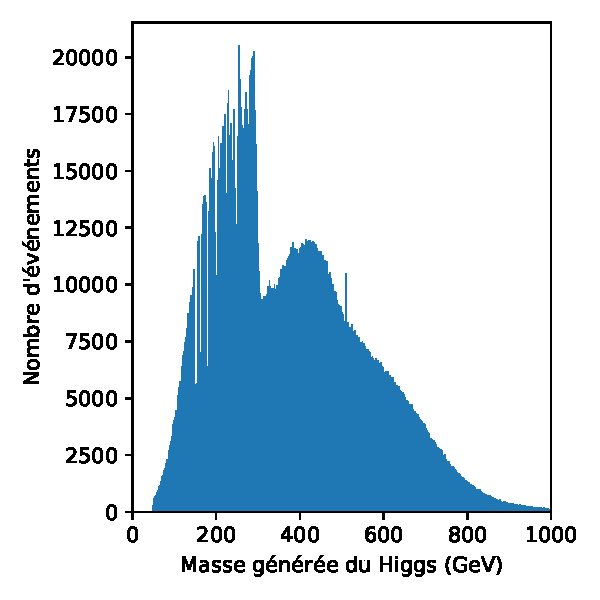
\includegraphics[width=.45\textwidth]{\PhDthesisdir/plots_and_images/my_plots/ML/from_ML_plots/FastSim_NanoAOD_to_NN/ALL_PU2017/plots_Htt_merged_NanoAODSIM_ALL_PU2017-DeepTau/distribution-inclusive-Higgs_mass_gen-raw-all_events.pdf}}
\hfill
\subcaptionbox{Distribution pondérée pour les événements d'entraînement.\label{subfig-distribution-inclusive-Higgs_mass_gen-weighted-is_train}}[0.45\textwidth]
{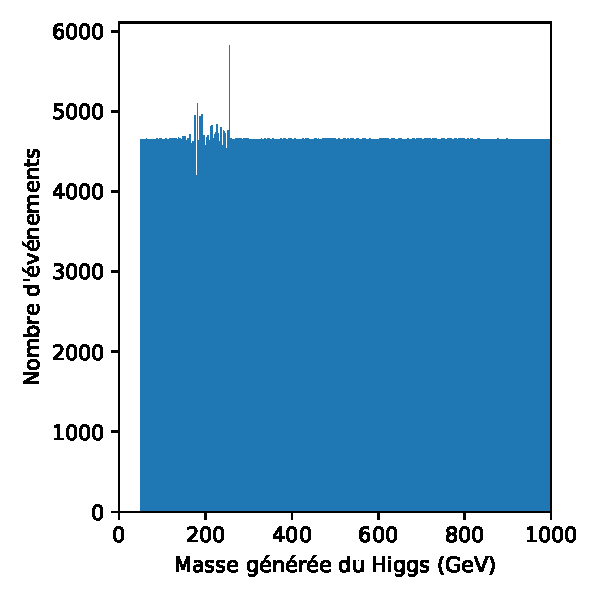
\includegraphics[width=.45\textwidth]{\PhDthesisdir/plots_and_images/my_plots/ML/from_ML_plots/FastSim_NanoAOD_to_NN/ALL_PU2017/plots_Htt_merged_NanoAODSIM_ALL_PU2017-DeepTau/distribution-inclusive-Higgs_mass_gen-weighted-is_train.pdf}}

\caption[Distributions de la masse générée de \higgsML.]{Distributions de la masse générée de \higgsML.}
\label{fig-distribution-inclusive-Higgs_mass_gen-raw-all_events}
\end{figure}
La largeur à \SI{800}{\GeV} est ainsi d'environ \SI{300}{\GeV}.
Le réglage $m_{\higgsML} = \SI{800}{\GeV}$ donne donc des événements contenant un boson dont la masse effective se situe entre \num{500} et \SI{1100}{\GeV}, d'où la queue de la distribution observée à haute masse sur la figure~\ref{subfig-distribution-inclusive-Higgs_mass_gen-raw-all_events}.
À basse masse en revanche, la largeur est inférieure à \SI{100}{\MeV}, cet effet n'est donc pas présent.
La cible du modèle est la masse effective du boson.
Les événements retenus dans la suite sont ceux où celle-ci se situe bien entre \num{50} et \SI{800}{\GeV},
d'où la disparition de la queue à haute masse sur la figure~\ref{subfig-distribution-inclusive-Higgs_mass_gen-weighted-is_train}.
\par
Ces événements sont de plus séparés en trois groupes selon les proportions suivantes:
\begin{itemize}
\item \SI{70}{\%} pour l'entraînement. Ce sont ces événements que les modèles pourront exploiter afin d'apprendre à prédire correctement $m_{\higgsML}$;
\item \SI{20}{\%} pour la validation. Ces événements permettent de vérifier qu'il n'y a pas de surentraînement, \ie\ que le modèle ne se spécialise pas vis-à-vis du jeu d'entraînement;
\item \SI{10}{\%} pour les tests. Ces événements ne sont pas utilisés lors des entraînements et permettent donc de tester les modèles sur des données inédites. Sauf contre-indication, les figures sont toutes obtenues avec ce groupe d'événements.
\end{itemize}
La répartition des événements dans ces trois groupes est faite de manière aléatoire.
\par
Afin de réaliser un entraînement équitable entre les différentes valeurs de $m_{\higgsML}$, un poids est associé à chaque événement de manière à ce que la distribution pondérée de $m_{\higgsML}$ soit plate dans chacun des trois groupes précédemment définis.
Cette distribution sur les événements utilisés pour l'entraînement des modèles est représentée sur la figure~\ref{subfig-distribution-inclusive-Higgs_mass_gen-weighted-is_train}.
\subsection{Cible et variables d'entrée des modèles}\label{chapter-ML-section-evt_gen-inputs}
La cible des modèles est la masse de la particule générée \higgsML\ se désintégrant en paire de leptons~\tau.
Un tel événement est illustré sur la figure~\ref{fig-model_inputs-fgraph-H-BBtautau_mutau_small}.
Les variables d'entrée doivent être des observables accessibles expérimentalement,
\ie\ issues de la reconstruction des événements présentée dans le chapitre~\refChLHCCMS.
\begin{figure}[h]
\centering
{\def\Higgs{\higgsML}\begin{fmffile}{H-tautau_mutau_small}\fmfstraight
\begin{fmfchar*}(50,25)
  \fmfleft{a,g1,b,c,g2,d}
  \fmfright{nu1,upq,doq,muout,antinumu,nu2}
  
  \fmf{gluon}{g1,g1loop}
  \fmf{gluon}{g2,g2loop}
  \fmf{phantom, tension=.2}{g1loop,upq}
  \fmf{phantom, tension=.2}{g2loop,antinumu}
  \fmffreeze
  \fmf{fermion}{g1loop,hloop,g2loop,g1loop}
  \fmf{fermion}{g2loop,g1loop}
  \fmf{dashes, label=$\Hn$, l.side=left, tension=1}{hloop,v}
  \fmf{phantom, tension=.2}{nu1,v,nu2}
  \fmffreeze
  
  \fmf{fermion, label=$\antitau$, l.side=left, tension=4}{t1d,v}
  \fmf{fermion, label=$\leptau$, l.side=left, tension=4}{v,t2d}
  \fmf{fermion, tension=3}{nu1,t1d}
  \fmf{boson, l.side=left, tension=2}{t1d,W1d}
  \fmf{phantom}{doq,W1d,upq}
  \fmf{fermion, tension=3}{t2d,nu2}
  \fmf{boson, tension=2}{t2d,W2d}
  \fmf{fermion}{antinumu,W2d,muout}
  \fmffreeze
  \fmf{plain}{W1d,upq}
  
  \fmflabel{\gluon}{g1}
  \fmflabel{\gluon}{g2}
  
  \fmflabel{{\color{ltcolorgray2}$\antinutau$}}{nu1}
  \fmflabel{{\color{ltcolorgray2}$\nutau$}}{nu2}
  \fmflabel{{\color{\muoncolor}$\muon$}}{muout}
  \fmflabel{{\color{ltcolorgray2}$\antinumu$}}{antinumu}
  \fmflabel{{\color{\tauhcolor}$\tauh$}}{upq}
  \fmfdot{g1loop,hloop,g2loop,v,t1d,t2d,W2d}
  \fmfblob{.07w}{W1d}
\end{fmfchar*}
\end{fmffile}
}
\caption[Diagramme de Feynman des événements d'entraînement des modèles.]{Diagramme de Feynman des événements d'entraînement des modèles dans le cas du canal \mu\tauh.}
\label{fig-model_inputs-fgraph-H-BBtautau_mutau_small}
\end{figure}
\par
Les variables considérées sont:
\begin{itemize}
\item les impulsions de $L_1$ et $L_2$ les produits de désintégration visibles des~\tau,
\ie\ le muon et le \tauh\ dans l'exemple de la figure~\ref{fig-model_inputs-fgraph-H-BBtautau_mutau_small}:\\
$\pT^{L_1}$, $\eta^{L_1}$, $\phi^{L_1}$,
$\pT^{L_2}$, $\eta^{L_2}$, $\phi^{L_2}$;
\item l'énergie transverse manquante pour rendre compte de la présence des neutrinos:\\
\MET, $\phi^{\MET}$, obtenus par l'algorithme \PUPPI~\cite{PUPPI};
\item la matrice $M$ de covariance de \MET, rendant compte de l'incertitude sur la mesure de \MET:\\
$M_{xx}$, $M_{xy}$, $M_{yy}$;
\item le nombre attendu de neutrinos lié à l'état final identifié \Nnu,
déterminé à partir du canal obtenu par la sélection des événements, \ie\ sans utilisation des informations générées;
\item les masses transverses
$\mT {(L_1,\MET)}$,
$\mT {(L_2,\MET)}$ et
$\mT {(L_1,L_2)}$
définies par
\begin{equation}
\mT {(A,B)} = \sqrt{2 \, \pT^{A} \, \pT^{B} \, (1-\cos(\phi^A-\phi^B))}
\mend[;]
\end{equation}
\item la masse transverse totale \mTtot\ définie par
\begin{equation}
\mTtot = \sqrt{\mT^2 {(L_1,\MET)} + \mT^2 {(L_2,\MET)} + \mT^2 {(L_1,L_2)}}
\mend[;]
\end{equation}
\item les impulsions des deux jets principaux (de plus haut \pT) présents dans l'événement:\\
$\pT^\text{jet 1}$, $\eta^\text{jet 1}$, $\phi^\text{jet 1}$,
$\pT^\text{jet 2}$, $\eta^\text{jet 2}$, $\phi^\text{jet 2}$;
\item l'Activité Hadronique Additionnelle (AHA), définie par la somme des impulsions des jets autres que les deux principaux:\\
$\pT^{\AddHadAct}$, $\eta^{\AddHadAct}$, $\phi^{\AddHadAct}$ avec
\begin{equation}
\vec{p}^{\AddHadAct} = \sum_\text{jet $i$, $i > 2$} \vec{p}^\text{jet $i$}
\mend[;]
\end{equation}
\item la quantité de jets utilisés pour déterminer $\vec{p}^{\AddHadAct}$, \Njetsr;
\item le nombre de vertex principaux d'empilement, \Npu.
\end{itemize}
Des modèles sont entraînés sur l'ensemble de ces 27 variables ainsi que sur des sous-ensembles de cette liste.